\documentclass[border = 1cm, convert, preview, varwidth]{standalone}

% mathematics
\usepackage{amsmath}

% tikz
\usepackage{tikz}
\usetikzlibrary{arrows}
\usetikzlibrary{automata}
\usetikzlibrary{positioning}
\tikzset{
  ->,
  >=stealth',
  node distance = 2cm,
}

% document
\begin{document}

\begin{figure}
  \centering
  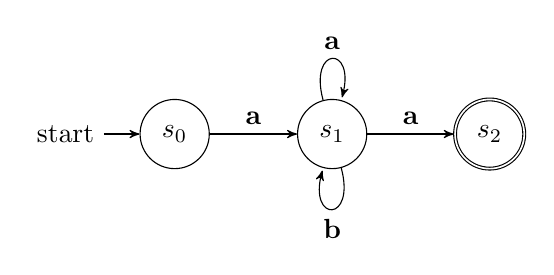
\begin{tikzpicture}
    \node [state, initial] (s0) {$s_0$};
    \node [state, right of = s0] (s1) {$s_1$};
    \node [state, accepting, right of = s1] (s2) {$s_2$};
    \draw (s0) edge [above] node {\textbf a} (s1);
    \draw (s1) edge [loop above] node {\textbf a} (s1);
    \draw (s1) edge [loop below] node {\textbf b} (s1);
    \draw (s1) edge [above] node {\textbf a} (s2);
  \end{tikzpicture}
  \caption{\textbf{a ( a \textbar \, b ) * b}}
\end{figure}

\begin{figure}
  \centering
  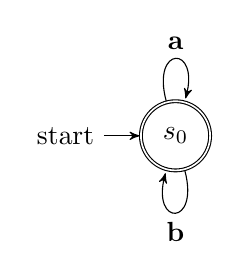
\begin{tikzpicture}
    \node [state, initial, accepting] (s0) {$s_0$};
    \draw (s0) edge [loop above] node {\textbf a} (s0);
    \draw (s0) edge [loop below] node {\textbf b} (s0);
  \end{tikzpicture}
  \caption{\textbf{( ( \(\boldsymbol\epsilon\) \textbar \, a ) b * ) *}}
\end{figure}

\begin{figure}
  \centering
  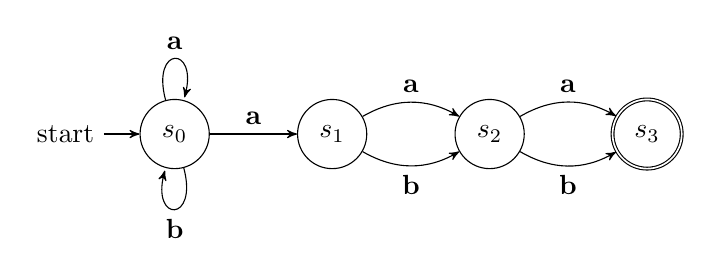
\begin{tikzpicture}
    \node [state, initial] (s0) {$s_0$};
    \node [state, right of = s0] (s1) {$s_1$};
    \node [state, right of = s1] (s2) {$s_2$};
    \node [state, accepting, right of = s2] (s3) {$s_3$};
    \draw (s0) edge [loop above] node {\textbf a} (s0);
    \draw (s0) edge [loop below] node {\textbf b} (s0);
    \draw (s0) edge [above] node {\textbf a} (s1);
    \draw (s1) edge [above, bend left] node {\textbf a} (s2);
    \draw (s1) edge [below, bend right] node {\textbf b} (s2);
    \draw (s2) edge [above, bend left] node {\textbf a} (s3);
    \draw (s2) edge [below, bend right] node {\textbf b} (s3);
  \end{tikzpicture}
  \caption{\textbf{( a \textbar \, b ) * a ( a \textbar \, b ) ( a \textbar \, b )}}
\end{figure}

\begin{figure}
  \centering
  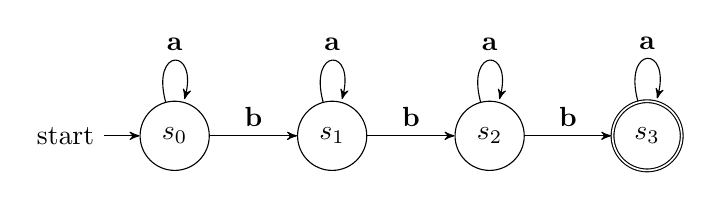
\begin{tikzpicture}
    \node [state, initial] (s0) {$s_0$};
    \node [state, right of = s0] (s1) {$s_1$};
    \node [state, right of = s1] (s2) {$s_2$};
    \node [state, accepting, right of = s2] (s3) {$s_3$};
    \draw (s0) edge [loop above] node {\textbf a} (s0);
    \draw (s0) edge [above] node {\textbf b} (s1);
    \draw (s1) edge [loop above] node {\textbf a} (s1);
    \draw (s1) edge [above] node {\textbf b} (s2);
    \draw (s2) edge [loop above] node {\textbf a} (s2);
    \draw (s2) edge [above] node {\textbf b} (s3);
    \draw (s3) edge [loop above] node {\textbf a} (s3);
  \end{tikzpicture}
  \caption{\textbf{a * b a * b a * b a *}}
\end{figure}

\begin{figure}
  \centering
  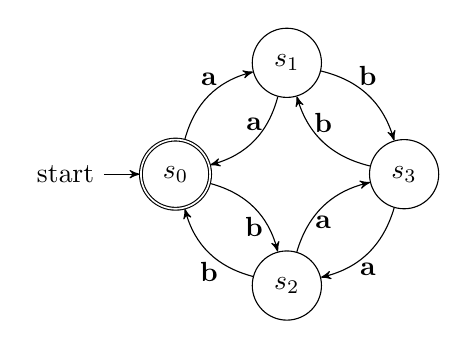
\begin{tikzpicture}
    \node [state, initial, accepting] (s0) {$s_0$};
    \node [state, above right of = s0] (s1) {$s_1$};
    \node [state, below right of = s0] (s2) {$s_2$};
    \node [state, right = 2cm of s0] (s3) {$s_3$};
    \draw (s0) edge [above, bend left] node {\textbf{a}} (s1);
    \draw (s1) edge [above, bend left] node {\textbf{a}} (s0);
    \draw (s0) edge [below, bend left] node {\textbf{b}} (s2);
    \draw (s2) edge [below, bend left] node {\textbf{b}} (s0);
    \draw (s1) edge [above, bend left] node {\textbf{b}} (s3);
    \draw (s3) edge [above, bend left] node {\textbf{b}} (s1);
    \draw (s2) edge [below, bend left] node {\textbf{a}} (s3);
    \draw (s3) edge [below, bend left] node {\textbf{a}} (s2);
  \end{tikzpicture}
  \caption{\textbf{(aa\textbar bb)*((ab\textbar ba)(aa\textbar bb)*(ab\textbar ba)(aa\textbar bb)*)*}}
\end{figure}

\end{document}
